% -*- root: ../Crypto.tex -*-
\section{Hoja 1}
\begin{problem}[1]
	Un general espartano recibe el siguiente mensaje de un amigo de Cantoblanco:


	SONFAUHPINPEOCTOHRIANEQLSGCUTUOHEEEQOENRUBSETEIDRELEIT

	¿Qué dice el mensaje?

	\solution
	\doneby{Jorge}

	Si consiguiéramos una escítala cuyo diámetro hiciera que entraran 5 letras por fila conseguiríamos el mensaje:

	SUPONGOQUELOHEHECHOBIENPORQUEESDIFICILTENERTANTASUERTE

\end{problem}

\begin{problem}[2]
	Recibes el mensaje VEILRÑW, cifrado usando una clave de Cesar en el alfabeto castellano de 27 letras (con Ñ y W). Lee el mensaje, da las transformaciones para cifrar y descifrar, y cifra el mensaje GRACIAS utilizando la clave correspondiente.

	\solution
	\doneby{Jorge}

	Usando la transformación:
	\[\appl{f_{17}}{ℤ/27}{ℤ/27}\]
	\[f_{17}(x) = x + 17\]

	Se consigue $f_{17}(\{V,E,I,L,R,Ñ,W\}) = \{M,U,Y,B,I,E,N\}$.

	De modo que para cifrar nos basta:
	\[f_{17}^{-1}(x) = f_{-17}(x) = f_{10}(x)\]
	\[f_{10}(\{G,R,A,C,I,A,S\}) = \{P,B,K,M,R,K,C\}\]
\end{problem}

\begin{problem}[3]
	Utilizando el análisis de frecuencias, descifra el siguiente mensaje, del que sabes que está escrito en inglés (26 letras, con W pero sin Ñ) y que ha sido cifrado con una clave de Cesar:
	PXPXKXENVDRUXVTNLXHYMXGMAXYKXJNXGVRFXMAHWGXXWLEHGZXKVBIAXKMXQM

	\solution
	\doneby{Jorge}

	Al hacer el análisis de frecuencias se obtiene:

	\begin{center}
		\begin{tabular}{ l l }
			P & 0.03225806451612903 \\
			X & 0.24193548387096775 \\
			K & 0.06451612903225806 \\
			E & 0.03225806451612903 \\
			N & 0.04838709677419355 \\
			V & 0.06451612903225806 \\
			D & 0.016129032258064516 \\
			R & 0.03225806451612903 \\
			U & 0.016129032258064516 \\
			T & 0.016129032258064516 \\
			L & 0.03225806451612903 \\
			H & 0.04838709677419355 \\
			Y & 0.03225806451612903 \\
			M & 0.08064516129032258 \\
			G & 0.06451612903225806 \\
			A & 0.04838709677419355 \\
			J & 0.016129032258064516 \\
			F & 0.016129032258064516 \\
			W & 0.03225806451612903 \\
			Z & 0.016129032258064516 \\
			B & 0.016129032258064516 \\
			I & 0.016129032258064516 \\
			Q & 0.016129032258064516
		\end{tabular}
	\end{center}

	Se puede ver que la más frecuente entre todas es la letra X. Si tomamos como letra más usada del ingés la E (en vez de la T) se obtiene el mensaje:

	WEWERELUCKYBECAUSEOFTENTHEFREQUENCYMETHODNEEDSLONGERCIPHERTEXT

	Gracias a la transformación $f_{7}(x) = x + 7$.
\end{problem}

\begin{problem}[4]
	La distribución de frecuencias (en porcentaje) en castellano de las 26 letras (es decir, sin W) es aproximadamente la siguiente.

	\begin{tabular}{c c c c c c c c c c c c c c c c c c c c c c c c c c c}
		A & B & C & D & E & F & G & H & I & J & K & L & M \\
		12,6 & 1,0 & 5,1 & 5,7 & 13,7 & 0,9 & 0,8 & 0,5 & 7,0 & 0,2 & 0,0 & 4,6 & 3,2 \\
		N & Ñ & O & P & Q & R & S & T & U & V & X & Y & Z \\
		7,0 & 0,1 & 8,8 & 2,9 & 1,1 & 6,6 & 7,2 & 5,1 & 3,9 & 0,8 & 0,1 & 0,6 & 0,3
	\end{tabular}

	Recibes un mensaje escrito en castellano (con ese alfabeto) que ha sido cifrado con el criptosistema de Cesar. Las dos letras más frecuentes en el texto cifrado son, por ese orden, la J y la N. Deduce razonadamente cual puede haber sido la clave utilizada para cifrar.

	\solution
	\doneby{Jorge}

	Lo lógico sería que las letras más frecuentes en el alfabeto se correspondieran con las más correspondientes en el mensaje, de modo que lo primero que a uno se le viene a la cabeza es corresponder la J (la más frecuente en el mensaje) con la E (la más frecuente en el alfabeto). Esto viene a ser la transformación $f_{-5}=f_{21}$, la cual manda la N (la segunda más frecuente en el mensaje) a la I (que no es la segunda más frecuente en el español).

	De modo que igual la segunda más frecuente en el mensaje es la que se corresponde con la más frecuente en el alfabeto ($f_{-9}=f_{17}$). Con esta transformación se consigue:
	\[f_{17}(J)=A\]
	\[f_{17}(N)=E\]
	Lo cual es más coherente, ya que hace una correspondencia entre las 2 letras más frecuentes del alfabeto (la E y la A) con las 2 más frecuentes del mensaje.
\end{problem}

\begin{problem}[5]
	Interceptamos un mensaje en el que dos profesores hablan de las asignaturas del plan de estudios de Matemáticas. El mensaje es el siguiente:

	DONQONHOSDGXQKCHDKSNSJSDOQOBDCUQ

	Sabemos que el mensaje ha sido cifrado utilizando una sustitución simple en el alfabeto castellano de 27 letras (con Ñ y W), y sospechamos que en el mensaje original aparecía la palabra CALCULO. Lee el mensaje.

	\solution
	\doneby{Jorge}

	Haciendo el análisis de frecuencias del mensaje interceptado se obtiene:

	\begin{center}
		\begin{tabular}{l l}
			D & 0.15625 \\
			O & 0.15625 \\
			N & 0.09375 \\
			Q & 0.125 \\
			H & 0.0625 \\
			S & 0.125 \\
			G & 0.03125 \\
			X & 0.03125 \\
			K & 0.0625 \\
			C & 0.0625 \\
			J & 0.03125 \\
			B & 0.03125 \\
			U & 0.03125
		\end{tabular}
	\end{center}

	Dentro del mensaje interceptado CALCULO se corresponde con NQONHOS, para darse cuenta basta con fijarse que hayan dos pares de letras iguales al igual que pasa en CALCULO. Con dicha correspondencia de letras tenemos (mostramos el mensaje cortado en 2, donde la fila de debajo de cada trozo se corresponde con lo que llevamos descifrado):

	\begin{center}
		\begin{tabular}{c c c c c c c c c c c c c c c c}
			D & O & N & Q & O & N & H & O & S & D & G & X & Q & K & C & H \\
			\_ & L & C & A & L & C & U & L & O & \_ & \_ & \_ & A & \_ & \_ & U
		\end{tabular}
	\end{center}

	\begin{center}
		\begin{tabular}{c c c c c c c c c c c c c c c c}
			D & K & S & N & S & J & S & D & O & Q & O & B & D & C & U & Q \\
			\_ & \_ & O & \_ & O & \_ & O & \_ & L & A & L & \_ & \_ & \_ & \_ & A
		\end{tabular}
	\end{center}

	Puesto que el análisis de frecuencias nos dice que la D es la letra que más aparece, probaremos a corresponderla con la letra E:

	\begin{center}
		\begin{tabular}{c c c c c c c c c c c c c c c c}
			D & O & N & Q & O & N & H & O & S & D & G & X & Q & K & C & H \\
			E & L & C & A & L & C & U & L & O & E & \_ & \_ & A & \_ & \_ & U
		\end{tabular}
	\end{center}

	\begin{center}
		\begin{tabular}{c c c c c c c c c c c c c c c c}
			D & K & S & N & S & J & S & D & O & Q & O & B & D & C & U & Q \\
			E & \_ & O & \_ & O & \_ & O & E & L & A & L & \_ & E & \_ & \_ & A
		\end{tabular}
	\end{center}

	Fijándonos en que la K y la C son las siguientes letras con mayor frecuencia, y que de entre las no utilizadas del alfabeto, la S y N son las siguientes que tienen más frecuencia en español. Probando se llega a que la K va a la N, y la C a la B.

	\begin{center}
		\begin{tabular}{c c c c c c c c c c c c c c c c}
			D & O & N & Q & O & N & H & O & S & D & G & X & Q & K & C & H \\
			E & L & C & A & L & C & U & L & O & E & \_ & \_ & A & N & B & U
		\end{tabular}
	\end{center}

	\begin{center}
		\begin{tabular}{c c c c c c c c c c c c c c c c}
			D & K & S & N & S & J & S & D & O & Q & O & B & D & C & U & Q \\
			E & N & O & \_ & O & \_ & O & E & L & A & L & \_ & E & B & \_ & A
		\end{tabular}
	\end{center}

	Llegados a este punto, somos capaces de adivinar que lo que pone el mensaje es:

	EL CALCULO ES TAN BUENO COMO EL ALGEBRA
\end{problem}


\begin{problem}[6]
	Interceptamos cuatro mensajes cifrados. Sabemos que tanto los mensajes en claro como los mensajes cifrados han sido escritos utilizando el alfabeto inglés de 26 letras. Las frecuencias con que cada letra aparece en cada mensaje son las siguientes:

	\begin{center}
		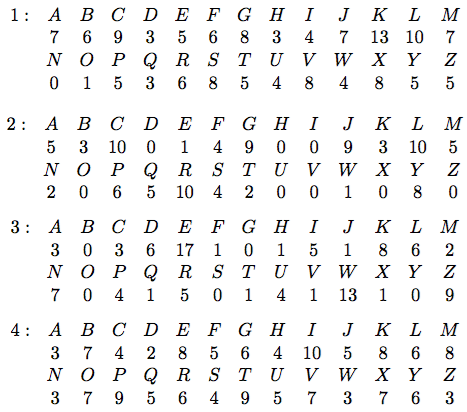
\includegraphics[width=0.5\textwidth]{img/freqsEj1_6}
	\end{center}

	¿Cuáles de los mensajes es razonable pensar que han sido cifrados utilizando sustituciones simples sobre letras?

	\solution
	\doneby{Pedro}

	Lo único que podemos hacer es fijarnos en las frecuencias de las diferentes letras y ver en qué mensajes las letras tienen unas frecuencias similares a las del inglés.

	Basándonos en la tabla de frecuencias de moodle podemos agrupar las letras del alfabeto inglés según la frecuencia con que se usan (en inglés y en cada uno de los mensajes interceptados).

	Si la columna de un mensaje se asemeja a la segunda columna, ese mensaje tendrá alta probabilidad de haber sido cifrado empleando una sustitución simple sobre letras.

	\begin{center}
	\begin{tabular}{| c | c || c | c | c | c |}
	\hline
	\textbf{Porcentaje} & \textbf{Nº Ingles} & \textbf{Nº M1} & \textbf{Nº M2} & \textbf{Nº M3} & \textbf{Nº M4} \\
	\hline
	0-2 & 10 & 2 & 9 & 12 & 0\\
	\hline
	2-4 & 6 & 3 & 4 & 3 & 5 \\
	\hline
	4-6 & 1 & 8 & 5 & 3 & 7 \\
	\hline
	6-8 & 7 & 6 & 1 & 3 & 8 \\
	\hline
	8-10 & 1 & 5 & 3 & 2 & 5 \\
	\hline
	>10 & 1 & 2 & 3 & 2 & 1 \\
	\hline
	\end{tabular}
	\end{center}

	Antes de nada hay que comentar que no sabemos qué longitud tenía cada mensaje por lo que tampoco sabemos cómo de válidas son las frecuencias calculadas. Por ello se ha tomado la decisión de agrupar las frecuencias por valores.

	Si sabemos que cada mensaje era un ``Los Pilares de la Tierra'' en inglés y cifrado, tendremos unas estimaciones de la frecuencia de cada letra muy muy buenas, por lo que podríamos agrupar las frecuencias por unidades.

	El primer y el último mensajes tienen muy pocas letras con baja frecuencia y demasiadas con frecuencia 8-10 por lo que parece razonable descartar la posibilidad de que hayan sido escritos en inglés.

	Entre el segundo y el tercero, el que más posibilidades tiene de haber sido escrito originalmente en inglés es el tercero, pues el segundo tiene muy pocas letras con frecuencia 6-8 y quizás demasiadas con frecuencias altas.

	Para el espía experto otra posibilidad sería estudiar la media y la varianza de la distribución de frecuencias en cada mensaje y apoyarse también en eso a la hora de tomar la decisión.
\end{problem}


\begin{problem}[7]
	En un alfabeto de 28 letras, las 27 del castellano y el espacio=27, utiliza la clave afíın sobre letras $f(m) = 13m + 9$ para cifrar el mensaje ``MUY BIEN''.

	\solution

	\doneby{Jorge}

	Utilizamos el $\_$ para representar el espacio y que este se vea claro.
	\[f(``MUY\_BIEN'')=``SXTRPW\_E''\]
\end{problem}


\begin{problem}[8]
	Sabemos que el enemigo está utilizando transformaciones afines sobre letras para cifrar mensajes escritos en inglés con el siguiente alfabeto de 37 letras: los números 0,...,9 que se codifican como ellos mismos; las letras A,…,Z (con W, sin Ñ), que corresponden a 10,…,35; y el espacio en blanco=36. Interceptamos el siguiente mensaje cifrado

	OH7F86BB46R3627O266BB9 (Atención, no hay ceros, sólo os)

	Sabiendo que el mensaje original acaba con la firma 007 (cero, cero, siete), ¿qué dice el mensaje?

	\solution
	\doneby{Jorge}

	La transformación afín será de la forma:
	\[ f_{a,b}(x) = ax+b \]

	Luego planteando un sistema de ecuaciones obtenemos a y b, sabemos que B=11:
	\[ f_{a,b}(11) = a·11 + b = 0\]
	\[ f_{a,b}(9)  = a·9  + b = 7 \]

	\[ b = -11a = 26a \]

	Luego
	\[ 9a + 26a = 35a = 7 \implies a = 15  \implies b = 20\]

	Aplicando $f_{a,b}$ al mensaje cifrado se obtiene:
	\begin{center}
		``AGENT 006 IS DEAD  007''
	\end{center}
\end{problem}


\begin{problem}[9]
	Una unidad de texto (en claro) m se dice que es fija para una transformación para cifrar si $f(m) = m$. Supongamos que estamos usando transformaciones afines sobre letras en un alfabeto de N letras, $f(m) = a · m + b$ con $a ≠ 1$.

	\begin{enumerate}
		\item Demostrar que si N es primo hay exactamente una letra fija.
		\item Demostrar que para N arbitrario cualquier transformación lineal (es decir, con b = 0) tiene al menos una letra fija, y que si N es par cualquier transformación lineal tiene al menos dos letras fijas.
		\item Dar un ejemplo de una transformación afín (para algún N) sin letras fijas.
	\end{enumerate}

	\solution
	\doneby{Jorge}
	\begin{enumerate}
		\item $m = a · m + b  \implies (a-1)·m + b = 0 \implies m = -(a-1)^{-1} · b$. En caso de que $N$ sea primo sabemos que existe $(a-1)^{-1}$, ya que en ese caso $U(ℤ/N)=ℤ/N$ y por tanto $(a-1) ∈ U(ℤ/N)$. Así que $m$ es único al quedar determinado por el producto de $(a-1)^{-1}$ y $b$.

		\item En caso de que $f(m) = a·m$ sabemos que siempre tendremos la letra fija asociada al 0 (ya que $f(0)=0$) independientemente de qué $N$ tengamos.

		Si $f(m) = a·m$ con $N$ par ($N=2M$), se cumple, además, que $f(M)=M$, ya que

		\[f(M)=M \iff aM = M \iff (a-1)M = 0 \iff 2M | (a-1)M \]

		Y puesto que $a$ debe ser unidad en $\ent_{2M}$, debe ser coprimo con $2M$ y, por tanto, impar. Por tanto, es claro que $(a-1)$ será par y, efectivamente $(a-1)M = k \cdot 2M$

		\item Para $N=2$ la transformación $f(x) = x + 1$ no deja letras fijas.
	\end{enumerate}
\end{problem}

\begin{problem}[10]
	Sea $A$ un anillo conmutativo con 1. Diremos que $a∈A$ es un divisor de 0 si existe $b∈A$, $b≠0$ y tal que $ab = 0$ (con esta definición, que no es la normal, 0 es un divisor de 0, pero no importa, simplifica los enunciados). Diremos que $a ∈ A$ es una unidad si existe $b ∈ A$ tal que $ab = 1$.

	\ppart Demostrar que $\left\{ \text{Unidades de } A \right\} ∩ \left\{ \text{Divisores de 0 en } A \right\} = \emptyset$
	\ppart Dado $a ∈ A$, definimos la aplicación ``multiplicar por $a$'', $\appl{m_a}{A}{A}$ como $m_a(x) = ax$. Caracterizar los divisores de 0 (o quizá los no divisores de 0) y las unidades de $A$ en términos de propiedades de la correspondiente aplicación $m_a$.
	\ppart Utilizar la caracterización anterior para demostrar que si $A$ es un anillo finito se tiene:

		\[\left\{ \text{Unidades de } A \right\} \cup \left\{ \text{Divisidores de 0 en } A \right\} = A\]

		(Esto generaliza lo que sucede en los anillos de congruencias $ℤ/Nℤ$.)
	\ppart Demostrar que la hipótesis de finitud es esencial en el apartado 3.

	\solution
	\doneby{Pedro}

	\spart
	Supongamos que tenemos un elemento $x$ que es unidad y divisor de 0 simultáneamente.

	En ese caso tendríamos que existen dos números $a$ y $b$, ambos distintos de 0, tales que: $ax = 0$ y $bx = 1$

	En esta situación podemos tomar la ecuación $bx=1$ y multiplicar por $a$ a ambos lados, con lo que mantenemos la igualdad, obteniendo:
	\[bx = 1 \iff abx = a \iff axb = a \iff 0 \cdot b = a \iff 0 = a\]

	Con lo que llegamos a una contradicción, pues dijimos que $a \neq 0$

	\spart

	Si tenemos que $a$ es un divisor de 0, habrá algún valor (distinto de 0) que nos llevará a 0, con lo que la función $f_a$ no será inyectiva.

	A raíz de esto podemos ver que si $a$ no es un divisor de 0, la función $m_a(x)=ax$ será inyectiva. Para comprobarlo basta con ver que:
	\[\forall x\neq y, \ ax=ay \implies a(x-y)=0 \implies a \text{ divisor de 0 ya que } x-y \neq 0\]
	lo que nos lleva a una contradicción.

	Por otro lado, si $a$ es una unidad, la función será sobreyectiva pues tendremos:
	\[\forall y \ ax = y \implies x = ya^{-1} \implies \exists x \tq m_a(x)=y\]

	Además, de esta misma fórmula podemos deducir que si no es unidad, no será sobreyectiva la función (no podremos llegar al 1, por ejemplo)

	\spart

	Si tenemos un elemento $a \in A$ que no es unidad ni divisor de 0 en $A$, tendremos que la función asociada $m_a$ será inyectiva pero no sobreyectiva.

	Si una función entre dos conjuntos finitos es inyectiva pero no sobreyectiva, esto implica que el conjunto de partida es menor que el de llegada. Pero por definición, la función $m_a$ va de un conjunto en si mismo, con lo que es imposible que sea inyectiva y no sobreyectiva.

	Por tanto es imposible que exista un $a$ como el que hemos definido. Es decir, tenemos demostrado que
	\[\left\{ \text{Unidades de } A \right\} \cup \left\{ \text{Divisidores de 0 en } A \right\} \supset A\]

	El otro sentido del contenido es trivial por la propia construcción del conjunto de unidades y de los divisores.

	\spart

	Si $A$ se tratase del anillo $(\ent, +, \cdot )$, dado $a=2$ podemos construir una aplicación $m_a$ que, como se probó en el apartado anterior, sería inyectiva pues 2 no es divisor de 0.

	Sin embargo, al no ser un cuerpo finito no hay problema en que una función vaya de un anillo en si mismo siendo inyectiva pero no sobreyectiva. Por tanto no podríamos deducir ninguna relación de contención.

	\doneby{Edu}

	\spart[a]

	Supongamos x $\in \text{Unidades de } A$ y $\exists y \neq 0 \tq x\cdot y = 0$, ie, x $\in \text{Divisores de 0 en } A$:
	\[ x \cdot y = 0 \implies x^{-1} \cdot x \cdot y = 0 \implies y = 0 \Rightarrow \Leftarrow \]
	{\bf Conclusión:} si x $\in \text{Unidades de } A \implies$ x $\not\in \text{Divisores de 0 en } A$

	Supongamos x $\in \text{Divisores de 0 en } A$, ie, $\exists y \neq 0 \tq x \cdot y = 0$ y supongamos $\exists z \neq 0 \tq x \cdot z = 1$:
	\[ x \cdot z = 1 \implies y \cdot x \cdot z = y \cdot 1 \implies 0 \cdot z = y \implies 0 = y \Rightarrow \Leftarrow \]
	{\bf Conclusión:} si x $\in \text{Divisores de 0 en } A  \implies$ x $\not\in \text{Unidades de } A$
	\newline\qed

	\spart[b]

	Si $m_a$ es inyectiva (y {\bf por ser A finito} entonces es sobreyectiva)

	$\implies \forall x,y \neq 0 \in A$, $m_a(x) = xa = ya = m_a(y) \implies x = y \implies $ a $\in $ unidades de A ya que, al ser {\bf sobreyectiva}, $\exists y \in A \tq a\cdot y = 1$.

	Si $m_a$ no es sobreyectiva, ie, GCD($m\cdot a$, |A|) $> 1$ para algún a, $\exists x,y \in A, x \neq y \tq$ $a \cdot x = a \cdot y \implies a (x - y) = 0 \implies a$ es divisor de 0.

	\spart[c]

	Como observación, diremos que si la afirmación es falsa, por el apartado 1, tiene que existir un $x$ que no pertenece a ninguno de los dos subconjuntos de A, lo cual es imposible por el apartado anterior: si $m_a$ es inyectiva, entonces $a$ es unidad, si $m_a$ no es sobreyectiva, $a$ es divisor de 0.
\newline\qed

	\spart[d]

	Leer la parte negrita del apartado B y convencerse de que no tiene por qué existir el inverso de $a$.

\end{problem}





\section{Control 1 (22-09-2014) Modelo A}
\begin{problem}[1]
Dado $N\geq 2$ y un elemento $a \in \ent_N$, consideramos la aplicación $\appl{m_a}{\ent_N}{\ent_N}$ tal que $m(x)=ax$.

Demostrar que son equivalentes:
\begin{enumerate}
\item $a$ es unidad en $\ent_N$
\item $a$ y $N$ son primos entre si.
\item $m_a$ es inyectiva
\item $m_a$ es sobreyectiva
\end{enumerate}

\solution
\doneby{Pedro}

Para demostrar que los enunciados son equivalentes vamos a demostrar una serie de implicaciones de modo que, al final, desde cualquiera de esas afirmaciones podamos llegar a cuaquier otra.

\begin{itemize}
\item \textbf{$1 \implies 2$}
Si $a$ es una unidad en $\ent_N$ sabemos que existe $c \in \ent_N$ tal que
\[ac = kN + 1\]

Supongamos ahora que $a$ y $N$ no son primos entre si, es decir,
\[\exists b \tq a = b \cdot a' \text{ y } N = b \cdot N'\]

Sustituyendo en la primera fórmula obtenemos
\[ba'c=bkN'+1 \iff b(a'c-kN')=1 \iff b \in U(\ent_N)\]

Pero está claro que $b$ no puede pertenecer a las unidades de $\ent_N$ ya que, siempre que $bc< N$ es claro que $bc \neq 1$ salvo que ambos sean 1 y, además:
\[\forall c \in \ent_N, \tq cb > N \iff cb = bN'α+bβ \text{ siendo } bβ < N\]
con lo que el resto nunca será 1.

\item \textbf{$2 \implies 3$}

Ahora tenemos $a$, $N$ tales que $(a,N)=1$ y queremos ver que la función $m_a$ es inyectiva.

Suponemos que no es inyectiva y que por tanto $\exists x,y \in \ent_N$ tales que $x \neq y$ y:
\[ax=ay \text{ mod } n \iff a(x-y)= 0 \ \text{mod } n \iff a(x-y) = c N\]

Pero, en caso de ser esto cierto, por definición, $a$ sería un divisor de $cN$ y, por tanto, $a$ divide a $c$ ya que estamos considerando $(a,N)=1$.

Si $a$ fuese divisor de $c$, podríamos escribir:
\[a(x-y)=kaN \iff (x-y) = kN\]
pero consideramos que $x$ y $y$ son dos elementos distintos de $\ent_N$ y, por tanto, su diferencia no puede ser múltiplo de $N$. Con lo que llegamos a una contradicción.

Por tanto no pueden existir $x$, $y$ como los descritos con lo que queda claro que la función es inyectiva.

\item \textbf{$3 \implies 4$}
Como estamos moviéndonos en un conjunto finito, si la función es inyectiva debe ser también sobreyectiva.

\item \textbf{$4 \implies 1$}

Si la función es sobreyectiva, entonces
\[\forall c \in \ent_N \exists b \in \ent_N \tq ab=c\]
en concreto esto es cierto para $c=1$ y por tanto $a$ tiene inverso, es decir, pertenece a las unidades de $\ent_N$

\end{itemize}

\end{problem}

\begin{problem}[2]
En un idioma que se escribe usando el mismo alfabeto que el inglés (26 letras), las letras más frecuentes son $B(20\%)$ y $Z(13\%)$, sin que ninguna de las demás letras tenga una frecuencia superior al $5\%$

Interceptamos un texto escrito en este idioma que ha sido cifrado usando un criptosistema afín sobre las letras vistas como elementos de $\ent_{26}$. Las letras más frecuentes en el mensaje cifrado resultan ser, por este orden, $H$ y $D$.

¿Qué letra en claro dirías que corresponde con la $E$ cifrada?

\solution
\doneby{Pedro}

Vamos a calcular directamente la función de descifrado, que será de la forma $f(m)=αm+β$. Sustituyendo los datos que tenemos nos queda el sistema:
\[\left\{
7α +β  = 1 \atop
3α + β = 25
\right. \implies 22α = 24 \implies 11α = 12 \]

Para resolver la ecuación tenemos que calcular el inverso de $11$ módulo 26. Para ello aplicamos el algoritmo de Euclides:
\[\begin{array}{l}
26 = 2 \cdot 11 +4\\
11 = 2 \cdot 4+ 3\\
4 = 1 \cdot 3 + 1
\end{array} \implies \begin{array}{l}
1 = 4 - 3 \\
3 = 11 - 2 \cdot 4 \implies 1 = 4 - 11 + 2 \cdot 4 = 3\cdot 4 -11 \\
4 = 26 -2 \cdot 11 \implies 1 = 3 \cdot 26 -6\cdot 11 - 11 = 3 \cdot 26 -7\cdot 11
\end{array}\]

Finalmente tenemos que $1 = 3\cdot 26 + 19 \cdot 11$, con lo que podemos resolver la ecuación, pues
\[α = 19 \cdot 12 = 20 \implies β = 17\]

Ahora podemos descifrar la letra $E$ obteniendo:
\[f(E)=f(4) = 15 = P\]
\end{problem}


